   

\documentclass[a4paper,12pt]{article}
\usepackage[english]{babel}
\usepackage{amsmath}
\usepackage{a4wide}

\usepackage{amsfonts}
\usepackage{amssymb}
\usepackage{graphicx}
\usepackage{color}
\usepackage{xcolor}
\usepackage{caption}
\usepackage{array}
\usepackage{pdfpages}
\usepackage{float}
\usepackage[round]{natbib}
\usepackage{multirow}
\usepackage{multicol}
\usepackage{amsxtra}
\usepackage{amsbsy}
\usepackage{bm}
\usepackage{accents}
\usepackage{chngcntr}
\usepackage{dcolumn}
\usepackage[none]{hyphenat}
\usepackage[affil-it]{authblk}
\usepackage{datetime}
\usepackage{footnote}
\makesavenoteenv{tabular}
\usepackage[flushleft]{threeparttable}
\usepackage[hyphens]{url}
\usepackage{placeins}
\usepackage{longtable}
\usepackage{booktabs}
\usepackage{setspace}
\usepackage{changepage}  
\usepackage{mathrsfs}
\usepackage{gensymb}

\usepackage{tabularx}
\usepackage[labelfont=bf]{caption}
\usepackage{titlesec}
\usepackage{endnotes}
\usepackage{csquotes}
\usepackage{euscript}
\usepackage{textcomp}
\usepackage{epstopdf}
\usepackage{graphicx}

\date{\normalsize{November 2018}}
\title{\Large \bf The Effects of Weather on Maize Yields: New Evidence from Kenya}
\author{Monika Novackova, Pedram Rowhani, Martin Todd, Dominic Kniveton}
\affil{\small{Department of Geography, University of Sussex, Falmer, UK}}


\parindent 0pt
\parskip 0.5em
\newcommand\starred[1]{\accentset{~~~~~\star}{#1}}


\begin{document}

\newdateformat{monthyeardate}{%
  \monthname[\THEMONTH], \THEYEAR}
  
  \interfootnotelinepenalty=10000

\makeatletter
\def\hlinewd#1{%
\noalign{\ifnum0=`}\fi\hrule \@height #1 %
\futurelet\reserved@a\@xhline}
\makeatother

\maketitle
\vfill
\epstopdfsetup{outdir=./}
\doublespacing

\begin{itemize}
\color{blue}
\item The title is provisional, we will decide about the final title when most of the paper will be written
\end{itemize}



\begin{abstract}
\noindent \textcolor{red}{..the full abstract to be written..} This paper contributes to better understanding of effects of drought on food security in Kenya which should lead to improving of early warning systems and food security. Our dataset consists of an yearly panel of $47$ counties of Kenya describing the period of 1981-2017.
\\
...Applying the linear mixed effects models, we found that...
\end{abstract}



\noindent \textbf{Keywords:}  Drought, Early warning systems, Food security, Food systems, Kenya, Mixed effects models\\




\newpage
\sloppy


\section{Introduction}\label{Introduction}


\begin{itemize}
\color{blue}
\item[] \textbf{Paragraph 1}

\begin{itemize}

\item Extreme weather causes disasters $\rightarrow$	 early warning systems have been developed
\end{itemize}
\item[] \textbf{Paragraph 2}
\begin{itemize}
\item What weather forecasts (measures) have been used in EWS? \textit{ref. litrature}
\begin{itemize}
\item Mostly seasonal precip. totals and temperature averages
\end{itemize}
\end{itemize}

\item[] \textbf{Paragraph 3} 
\begin{itemize}

\item Identify difference between hazard and disaster

\begin{itemize}
\item Not every hazard turns into disaster
\item For a hazard to become a disaster it needs to have \textbf{impact}
\item Here, we identify the key metrics which have impact on yield
\end{itemize}

\end{itemize}

\item[] \textbf{Paragraph 4}
\begin{itemize}
\item Crop yield versus climate forecasting
\end{itemize}


 \item[] \textbf{Paragraph 5}
\begin{itemize}
\item Aim of the paper:

\color{red}


In the light of these arguments, the goal of the present study is to develop a model which will utilize weather data to assess risk of drought and food security. In addition, we want to find out which particular features of climate or weather are the most important factors affecting the yields and food security. Are the average weather conditions the most important or is it the weather variability or length and number of dry spells during the growing season what matters the most? Answering these and other similar questions should help to improve food security and shift the focus from reactive to proactive approach in drought disaster risk management. We focus on Kenya utilizing an yearly panel of $47$ counties over the period of $1981-2017$. % mozna hodit tuhle vetu na zacatek 2.1. Measures of food security and drough
\color{black}
\end{itemize}
 
\end{itemize}
\section{Methods}\label{Methods}

\color{blue}

\textit{..this is a case study looking at Kenya...}


\subsection{Data}\label{Data}
\begin{itemize}
\item Source of the climate data: \cite{BOKU} (BOKU) and \cite{Berkeley}
\item Source of the yield data (Kenya MoA)
\end{itemize}

\color{black}
\subsection{Statistical approach}



% No need to write too many details (or a section) about measures of food security
% No need to describe all the weather measures/characteristics that we have calculated and/or tried to use and didn't work
\begin{itemize}
\color{blue}
\item \textit{We used commonly used measures of weather/drought (Only mention the significant weather measures/variables)}

\item Describe the temporal aggregation of the weather variables, seasons
\end{itemize}
\color{black}

\sloppy
Kenya consists of $47$ counties with semi-autonomous county governments  \citep{Barasa2017}. As a result of the high degree of county-level autonomy, the policies and regulations often differ across the counties, hence the effects of weather on crop yield are likely to be different across the counties. Therefore, following the standard methodology, we estimated a battery of linear mixed effects models (also known as mixed models) commonly used to analyse longitudinal data \citep{bates2000mixed}. Mixed models are suitable for analysis of panel data as they account for the panel structure of the dataset. These types of models include both fixed effects parameters and random effects. Fixed effects are analogous to parameters in a classical linear regression model and value of each effect is assumed to be fixed over all counties \citep{bates2010lme4}. On the other hand, random effects are unobserved random variables. There are at least three benefits of treating a set of parameters as a random sample from some distribution. \textit{(i)} Extrapolation of inference to a wider population \textit{(ii)} improved accounting for system uncertainty and \textit{(iii)} efficiency of estimation (\citealp{KERYch9, KERYch12}).

Formally, a linear mixed model can be described by the distribution of two vectors of random variables: the response $\mathscr{Y}$ and the vector of random effects $\mathscr{B}$. The distribution of $\mathscr{B}$ is multivariate normal and the conditional distribution of $\mathscr{Y}$ given $\mathscr{B}=\mathbf{b}$ is multivariate normal of a form (\citealp{bates2010lme4, KERYch9}):




\begin{equation}\label{MixedGeneral}
\begin{array}{lcl}

(\mathscr{Y}|\mathscr{B}=\mathbf{b})& \sim & \mathit{N}(\mathbf{X}\mathbf{\beta}+\mathbf{Z}\mathbf{b},\sigma^2\mathbf{I}),

\end{array}
\end{equation}

where $\mathbf{X}$ is an $n \times p$ model matrix of fixed effects, $\mathbf{\beta}$ is a $p$-dimensional fixed-effects parameter, $\mathbf{Z}$ is an $n \times q$ model matrix for the $q$-dimensional vector of random-effects variable $\mathscr{B}$ evaluated at $\mathbf{b}$ and $\sigma$ a scale factor. The distribution of $\mathscr{B}$ can be written as: 

\begin{equation}\label{ranefDist}
\mathscr{B} \sim \mathit{N}(0,\mathbf{\Sigma}),
\end{equation}

where $\mathbf{\Sigma}$ is a $q \times q$ positive semi-definite variance-covariance matrix.

\color{blue}
\begin{itemize}
\item Add a description of residual and other diagnostic tests (AIC, VIF, autocorrelation)
\item Describe the procedure that I have applied to find the preferred combination of fixed effects and random effects
\item Describe the procedure that I have applied to find the preferred way of modelling the  correlation structure in errors (ARMA errors)
\end{itemize}
\color{black}
\FloatBarrier




\section{Results}\label{Results}

\color{blue}
\begin{itemize}

\item Tables of estimates of the preferred specification which includes the significant weather variables (see the preliminary results in Table \ref{KenARe11}) 

\begin{itemize}
\item For all counties 
\item For Arid and semi-araid (ASAL) counties
\item For non-ASAL counties
\end{itemize}

\color{black}

{
\begin{threeparttable}
\singlespacing
\caption{\textit{\textbf{Mixed  effects model:} Log of maize yield and weather, ARMA(1,1) errors}}
%KEN11a  KEN11a_ASAL    KEN11a_nonASAL														
\label{KenARe11} 
\begin{footnotesize}
\begin{tabular}{llrlllr} 
\hline \vspace{-0.2cm} \\
\vspace{-0.2cm} \\
  \multicolumn{1}{l}{\vspace{0.1cm}\textbf{ }}  &\multicolumn{2}{c}{\textit{\textbf{All counties}}} &\multicolumn{2}{c}{\textit{\textbf{ASAL}}} &\multicolumn{2}{c}{\textit{\textbf{non-ASAL}}}\\
    \multicolumn{1}{l}{\vspace{0.1cm}\textbf{Fixed effects:}}&\boldsymbol{$exp(\beta)$}&\textbf{F-value\tnote{a}}%> anova(KEN11a, type='marginal')
    &\boldsymbol{$exp(\beta)$}&\textbf{F-value\tnote{a}}&\boldsymbol{$exp(\beta)$}&\textbf{F-value\tnote{a}}\\
 \hline 
\hline
\\
\vspace{-0.2cm}Intercept&$1.296^{***}$&$19.916$&$1.276^{*}$&$5.230$&$1.410^{**}$&$10.061$\\
  \\ \vspace{-0.2cm}Prec. total&$1.081^{*}$&$5.402$&$1.006^{}$&$0.022$&$1.278^{***}$&$19.386$\\
  \\
  \vspace{-0.2cm}Prec. total sq.&$0.973^{*}$&$4.289$&$1.004$&$0.051$&$0.880^{***}$&$23.747$\\
    \\ \vspace{-0.2cm}Prec. c. of var.&$0.924^{\bullet}$&$3.277$&$0.969$ &$0.246$&$0.909^{}$&$2.231$\\
  \\  \vspace{-0.2cm}Dry spell -length&$0.935^{*}$&$4.810$&$0.833^{**}$&$6.969$&$ 0.988^{}$&$0.163$\\
  \\ \vspace{-0.2cm}Dry spells 	$\geq$ 4 d.&$0.939^{*}$&$4.826$&$0.855^{**}$&$8.065$&$0.989^{}$&$0.096$\\
  \\ \vspace{-0.2cm}Temp. - average&$0.819^{***}$&$12.127$&$0.808^{*}$&$5.376$&$0.878$ $^{}$&$1.580$\\
  \\  \vspace{-0.2cm}Temp. std. dev.&$1.043^{\bullet}$&$3.125$&$1.039$&$0.558$&$1.059$ ${*}$&$5.640$\\
  \\
  \hline
\vspace{-0.2cm} \\
  \multicolumn{1}{l}{\textbf{Random effects:}}  & \\
\vspace{-0.2cm}
\\
\hline
\\
  \vspace{-0.2cm}Intercept\\
 \\ 
 \hline
\vspace{-0.2cm} \\
\textit{Number of observations:}  &\multicolumn{2}{c}{$1300$}&\multicolumn{2}{c}{$698$}&\multicolumn{2}{c}{$602$}\\
\vspace{-0.2cm}
\\  
  
  \hline
  \vspace{-0.2cm} \\

\hline
\vspace{-0.2cm}
\end{tabular} 
\end{footnotesize}
 \begin{tablenotes}
  \begin{footnotesize}
    \item \textit{Notes:} Standard errors in brackets; \hfill $^{\bullet}~p<0.1$; $^{*}~p<0.05$; $^{**}~p<0.01$; $^{***}~p<0.001$
        \begin{adjustwidth}{1cm}{} 
    \item[a] Marginal (type III) sum of squares. The F-statistics correspond to the sum of squares attributable to each fixed effect.
     \end{adjustwidth}
\singlespacing
  \end{footnotesize}
\end{tablenotes}
  \end{threeparttable} 
\par}
\linespread{1}


  \begin{figure}
   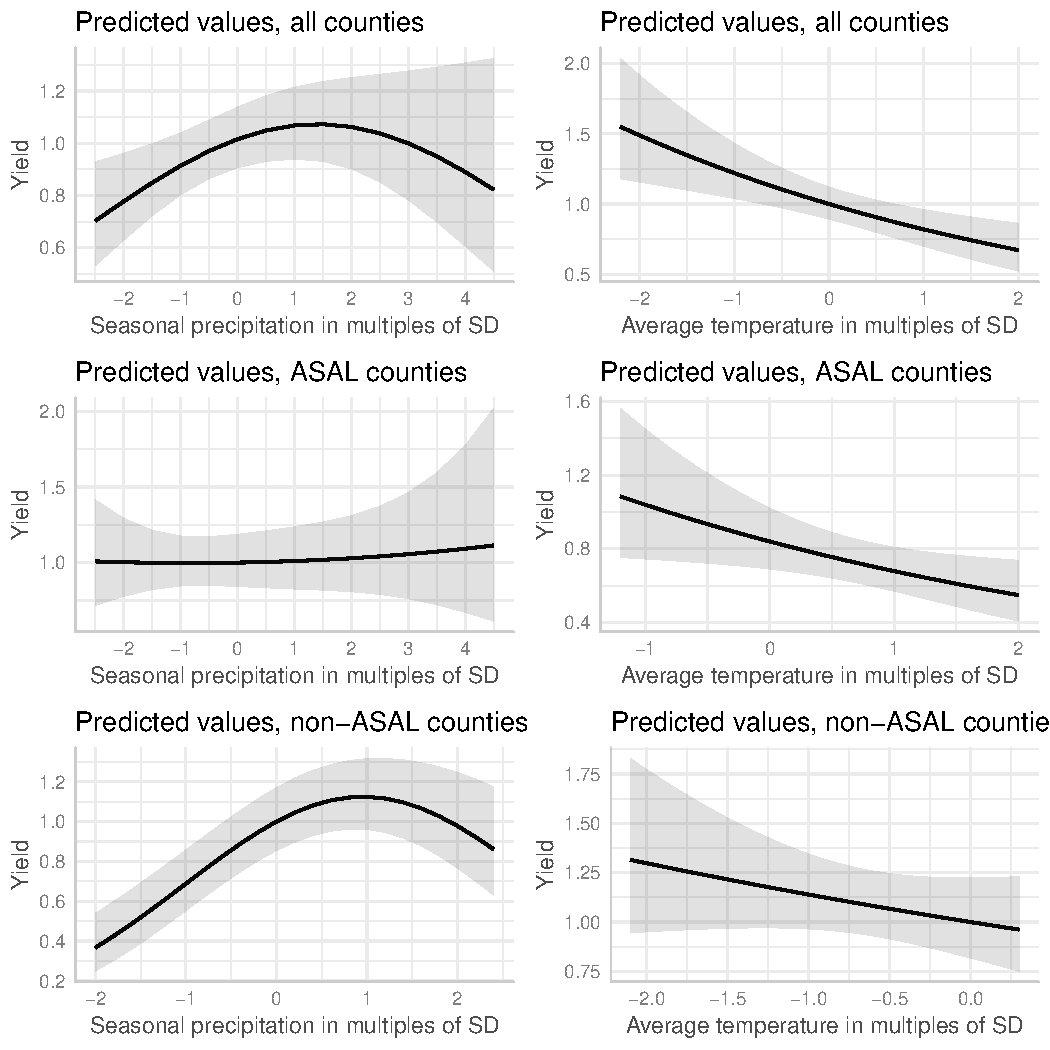
\includegraphics{marginalEffects.pdf}
\caption{Marginal effects of seasonal rainfall and temperature}\label{bar}
\end{figure}


\color{blue}




	
\item Verbal description and interpretation of the results. Discussing goodness of fit using various criteria such as AIC or alternatives to $R^2$.
%\item Possibly estimate simple regressions with the same explanatory variables as the preferred mixed effects specification. This would give us an approximation of $R^2$ which could be used to compare our models.

	%	\begin{itemize}%
		%	\item \textcolor{red}{Annemie has advised me that for a more precise approximation of $R^2$ we can estimate a simple regression of yields on the random intercepts (county level dummy variables) and then subtract the $R^2$ of this model from the $R^2$ of the simple regression with the explanatory variables of the preferred mixed models (the model described in the bullet point above). This would give us a percentage of yield variability explained by the weather measures not including the variability explained by the random intercepts.}
	%\end{itemize}
	
\item If we get the yield data for the period from $2015$ onwards: Out of sample predictions and comparison with the real data
\end{itemize}


\color{black}
\section{Discussion}\label{Discussion}

\color{red}
		


	\begin{itemize}
	\item There are many weather/climate characteristics (measures) which are important for yield, not only seasonal totals (averages)
	\item  Current weather and climate forecasts (in the context of disaster management) are mostly focused on totals in precipitation (and average temperature?) 
	\item There is a strong movement to shift the focus from forecasting merely weather/climate to forecast of weather/climate and its impacts
	
	\begin{itemize}
	\item[$\boldsymbol{\rightarrow}$] \textbf{We can stress the importance of focusing the forecast on the climate characteristics (or measures) which we find significant in our models}
\end{itemize}

	\item \textcolor{red}{Caveats}
	
	\begin{itemize}
	\item\textcolor{red}{ Yield data: Is the collection method consistent over time and space?}
	\item Livestock not explicitly taken into account
	\item Cropping calendar is likely to differ across the country 
	\item \textcolor{red}{Some more??}
	
	\end{itemize}
\end{itemize}
\color{black}



\section*{If time}\label{iftime:}
\color{violet}
\begin{itemize}
\item Estimates of future impacts and comparison of forecast accuracy of the base and preferred model
\begin{itemize}
\item The idea is to choose two points in time from within our period of data and imagine that we are in the earlier of the two time points. Now we want to make a prediction of yields for the later point in time. We will make two predictions: one using the base model (which only includes precipitation and temperature) and the other based on the preferred specification and we will compare their prediction accuracy. Here, we assume that predictions of the weather measures are available (the explanatory variables of our models). We can use real weather data instead of the forecast. This will demonstrate why it is important to not only forecast totals/means but also other characteristics (measures) of weather/climate.
		\item Accompany with a graph(s), possibly barplot(s)
\end{itemize}

\item Estimate a variant of the model which separates the effects of the seasons for ASAL counties (OND and MAM separately). If interesting show a table and discuss.

\item Show a variant of the model without the outliers. This could be presented either by a table in this section, a table in the Appendix or a table in a footnote. 

\item I can also estimate similar models for different important crops in Kenya (e.g. wheat, rice, sorghum or millet)


\end{itemize}
\color{black}
\FloatBarrier
\pagebreak





%TTTTTTTTTTTTTTTTTTTTTTTTTTTTTTTTTTTTTTTTTTTTTTTTTTTTTTTTTTTTTTTTTTTTTTTTTTTTTTTTTTTTTTTTTTTTTTTTTTTTTTTTTTTTTTTTTTTTTTTTTTTTTTTTTTTTTTTTTTTTTTTTTTTTTTTTTTTTTTT

%TTTTTTTTTTTTTTTTTTTTTTTTTTTTTTTTTTTTTTTTTTTTTTTTTTTTTTTTTTTTTTTTTTTTTTTTTTTTTTTTTTTTTTTTTTTTTTTTTTTTTTTTTTTTTTTTTTTTTTTTTTTTTTTTTTTTTTTTTTTTTTTTTTTTTTTTTTTTTTT

\makeatletter 
\renewcommand{\thesection}{\hspace*{-1.0em}}
\newpage
\linespread{1}

\bibliographystyle{ChicagoM}
%\bibliographystyle{apa}
\bibliography{referencesFS}

\newpage

\setcounter{table}{0} 
\makeatletter 
\renewcommand{\thetable}{A\@arabic \c@table} 
\FloatBarrier


\section{Appendix 1 Drought: definitions, measures and indices}
According to the international meteorological community, drought can be defined in several ways. In particular, drought is a \textit{'prolonged absence or marked deficiency of precipitation'}, a \textit{'deficiency of precipitation that results in water shortage for some activity or for some group'} or a \textit{'period of abnormally dry weather sufficiently prolonged for the lack of precipitation to cause a serious hydrological imbalance'} (\citealp{Heim2002, IPCCtrenberth}).
 \cite{AMS1997} has defined three types of droughts: \textit{(i)}~'Agricultural drought' which is defined in terms of moister deficits in upper layer of soil up to about one meter depth~\textit{(ii)} 'meteorological drought' which refers to prolonged deficit of precipitation and~\textit{(iii)} 'hydrological drought' which relates to low streamflow, lake and levels of groundwater. The  \cite{AMS1997} policy statement was later replaced by another statement \citep{AMS2013} which besides the three types of drought above, covers also the 'socioeconomic drought' which associates the supply and demand of some economic good with elements of meteorological, agricultural and hydrological drought (\citealt{Heim2002, IPCCtrenberth}).
 
\cite{wilhite1985} and \cite{wilhite2000} have distinguished two main categories of definitions of drought: \textit{(i)} conceptual and \textit{(ii)} operational. Conceptual definitions are dictionary types, usually defining boundaries of the concept of drought\footnote{An example of conceptual definition of drought is an 'extended period - a season, a year, or several years of deficient rainfall relative to the statistical multi-year mean for a region' \cite{schneider1996}.}. Operational definitions are essential for an effective early warning system. An example of operational definition of agricultural drought can be obtaining the rate of soil water depletion based on precipitation and evapotranspiration rates and expressing these relationships in terms of drought effects on plant behaviour \citep{wilhite2000}.

In order to compare severity of drought across different time periods or geographical locations a numerical measure turns out to be necessary. However, as a result of a large disagreement about a definition of drought, there is no single universal drought index. Instead of that a number of measures of drought has been developed (\citealp{ wilhite1985, wilhite2000, Heim2002}).

 
 
Examples of early measures of drought are \cite{wilhite1985}, \cite{munger1916}, \cite{blumenstock1942} or \cite{mcquigg1954}. \cite{munger1916} suggested to use length of period without $24$-h precipitation of $1.27$ mm. \cite{wilhite1985} is based on a measure of precipitation over a given time period. \cite{blumenstock1942} proposed to measure severity of drought as a length of drought in days where the end of a drought is defined by occurrence of $2.54$ mm of precipitation in $48$ hours. \cite{mcquigg1954} developed the Antecedent Precipitation Index (API) which is based on amount and timing of precipitation and it was used for forecasting of floods. Hence, the API is a reverse drought index.

The study of \cite{palmer1965} was a significant milestone in the history of quantification of drought severity. \cite{palmer1965} developed the Palmer Drought Severity Index (PDSI) using a complex water balance model. The PDSI is based on a hydrological accounting system, which incorporate antecedent precipitation, moisture supply and moisture demand (\citealp{Heim2002,palmer1965}). As the PDSI suffers from several weaknesses (for details see e.g. \citealt{Heim2002}), other indices were developed in the following decades. These include the standardized precipitation index (SPI) developed by \cite{SPI} and the standardized precipitation evapotranspiration index (SPEI) developed by \cite{SPEI}. The SPI specifies observed precipitation as a standardised departure from a chosen probability distribution which models the precipitation data. Values of SPI can be viewed as a multiple of standard deviations by which the observed amount of rainfall deviates from the long-term mean \citep{SPIonline}.\footnote{Can be created for various periods of 1-36 months, usually using monthly data.} The SPEI is similar to SPI, but unlike SPI, the SPEI includes the role of evapotranspiration (which captures increased temperature). It is based on water balance, therefore it can be compared to the self-calibrated PDSI \citep{SPEI}. 


\section{Appendix 3 Tables}







\end{document}
